\part{Esperienze didattiche} \label{parte:esperienze-didattiche}

\chapter{L'esplorazione di Marta} \label{cap:marta}

\section{Prologo}

Marta Veloce è una studentessa che ha frequentato il Laboratorio di Tecnologie
Didattiche nell'Anno Accademico 2016/17, giusto prima di laurearsi. L'11
novembre, dopo poco più di un mese dall'inizio del laboratorio, Marta mi
invia la seguente email con un elaborato molto interessante, che ha dato adito
a una serie di riflessioni e approfondimenti. Iniziamo la storia con l'email
inviata da Marta.

\begin{quote} Le scrivo perché ho provato a riflettere su alcune questioni,
	usando Logo, e ho sviluppato un breve percorso con alcuni "esercizi di
	creatività", come li ho chiamati io, eventualmente da poter svolgere
	con i bambini, basati sull'operazione di ripetizione di elementi per
	formare nuove immagini. Mi sono ispirata al libro di Munari\cite{Munari},
	"Fantasia"; bellissimo! A partire da questo, ho poi sviluppato alcune
	riflessioni, anche di tipo geometrico, che, devo essere sincera, mi
	hanno fatto un po' "impazzire"; ho raccolto alcune ipotesi e dati e,
	anche se non sono giunta a nessuna conclusione definitiva, ho comunque
	trovato alcuni aspetti interessanti, su cui magari poter riflettere. Le
	invio l'elaborato per email, perché ricordo che ci aveva chiesto di
	fare così nel caso in cui producessimo documenti pesanti e troppo
	lunghi da caricare su Moodle.    \end{quote}

Riporto qui di seguito l'elaborato, così come l'ho ricevuto da Marta.

\section{“Esercizi” di creatività – giocare con la ripetizioni in Logo}

Questo tipo di percorso prende avvio dalla lettura di un bellissimo testo di
Bruno Munari, Fantasia.  Il testo è proprio un elogio alla fantasia, rispetto
alla quale la creatività si configura come suo uso finalizzato. Una persona
colta senza fantasia, secondo Munari, è come un dizionario, pieno di parole ma
senza alcuna poesia. Una delle operazioni mentali della fantasia, basate sul
mettere in relazione i dati noti per creare qualcosa di nuovo, consiste nella
ripetizione di unità, senza alcuna variazione. Che cosa avviene se ripetiamo
alcuni oggetti più e più volte? Si è provato a dare una risposta, utilizzando
Logo e sfruttandone le grandi potenzialità grafiche: “A lui la precisione
tecnica, a noi la sperimentazione, la riflessione… e il divertimento!” Il
percorso non si limita a dare libero sfogo alla fantasia, ma si apre anche ad
alcune riflessioni geometriche e aritmetiche, che procedono mediante metodo
induttivo e secondo un approccio scientifico (osservazione-ipotesi-verifica).
Si è ipotizzato di lavorare con una classe di bambini di scuola primaria.

\subsection{Fase I}

Chiediamo ai bambini di costruire una casetta. Il primo dei comandi deve essere
“CLEARSCREEN”, così che si possa riavviare il programma tutte le volte che
vogliamo, facendo compiere sempre lo stesso movimento alla tartaruga.

\begin{minipage}{0.5\textwidth}
\begin{figure}[H]
   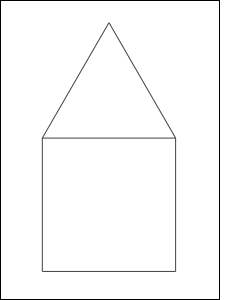
\includegraphics[width=5.0cm,trim=4 4 8 4,clip]{./images/marta/mar-1.png}
   \label{mar-1}
\end{figure}
\end{minipage} \hfill
\begin{minipage}{0.45\textwidth}
\begin{itemize}[itemsep=-3pt,parsep=2pt]
\item[] \hspace{0.5cm} CLEARSCREEN
\item[] \hspace{0.5cm} HOME 
\item[] \hspace{0.5cm} FORWARD 100
\item[] \hspace{0.5cm} RIGHT 90
\item[] \hspace{0.5cm} FORWARD 100
\item[] \hspace{0.5cm} RIGHT 90
\item[] \hspace{0.5cm} FORWARD 100
\item[] \hspace{0.5cm} RIGHT 90
\item[] \hspace{0.5cm} FORWARD 100
\item[] \hspace{0.5cm} RIGHT 90
\item[] \hspace{0.5cm} FORWARD 100
\item[] \hspace{0.5cm} RIGHT 30
\item[] \hspace{0.5cm} FORWARD 100
\item[] \hspace{0.5cm} RIGHT 120
\item[] \hspace{0.5cm} FORWARD 100
\end{itemize}
\end{minipage}

\subsection{Fase II}

Proviamo adesso ad eliminare il primo comando, “CLEARSCREEN”, e proviamo a riavviare il programma per due o più volte. Ci renderemo conto che, poiché adesso il disegno iniziale non viene cancellato, ogni volta che il programma si riavvia, la tartaruga traccia la stessa figura su quella precedente; si può osservare infatti, che, ad ogni riavvio, il tratto diventa sempre più spesso ed il colore nero si fa più intenso. Invitiamo i bambini a cliccare con il tasto sinistro del mouse sul disegno e a “spostarlo”; si renderanno subito conto che sul tracciato sono sovrapposte più casette che, se spostate a piacimento, possono costituire un bel quartiere!

\begin{minipage}{0.5\textwidth}
\begin{figure}[H]
   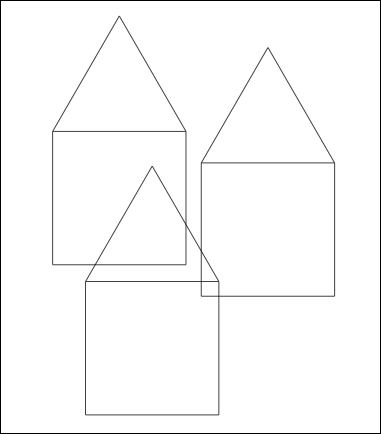
\includegraphics[width=5.0cm,trim=4 4 6 4,clip]{./images/marta/mar-2.png}
   \label{mar-2}
\end{figure}
\end{minipage} \hfill
\begin{minipage}{0.45\textwidth}
\begin{itemize}[itemsep=-3pt,parsep=2pt]
\item[] \hspace{0.5cm} HOME 
\item[] \hspace{0.5cm} FORWARD 100
\item[] \hspace{0.5cm} RIGHT 90
\item[] \hspace{0.5cm} FORWARD 100
\item[] \hspace{0.5cm} RIGHT 90
\item[] \hspace{0.5cm} FORWARD 100
\item[] \hspace{0.5cm} RIGHT 90
\item[] \hspace{0.5cm} FORWARD 100
\item[] \hspace{0.5cm} RIGHT 90
\item[] \hspace{0.5cm} FORWARD 100
\item[] \hspace{0.5cm} RIGHT 30
\item[] \hspace{0.5cm} FORWARD 100
\item[] \hspace{0.5cm} RIGHT 120
\item[] \hspace{0.5cm} FORWARD 100
\end{itemize}
\end{minipage}

\subsection{Fase III}

Proseguiamo in questo gioco creativo. Proviamo ad eliminare anche il comando
“HOME” posto in cima alle istruzioni e volto a far tornare ogni volta la
tartaruga in posizione iniziale. Che cosa accadrà? Stavolta, riavviando il
programma, la tartaruga esegue il medesimo movimento, partendo però dalla
posizione assunta in base all’ultimo comando. Essendo l’ultimo comando “FORWARD
100” e coincidendo questo con il movimento atto a descrivere l’ultimo lato del
triangolo-tetto, la tartaruga si trova disposta “a testa in giù”, orientata
verso una direzione a 30 gradi a sinistra rispetto alla verticale. Per
comprendere questo è necessario fare dei ragionamenti di tipo geometrico e
aritmetico: è necessario sottrarre dall’angolo piatto (formato dall’ultimo lato
del tetto e da un suo eventuale prolungamento) l’angolo di 150 gradi, formato
dalla somma dell’angolo interno del triangolo (60 gradi) e quello del quadrato
(90 gradi). Così facendo otteniamo il valore di 30 gradi.

Che cosa viene fuori se avviamo più volte il programma? Diamo il via
all’immaginazione: ognuno può vederci ciò che vuole! Qualcuno potrebbe vederci
una girandola, qualcun altro una stella, qualcuno un fiore!

\begin{minipage}{0.5\textwidth}
\begin{figure}[H]
   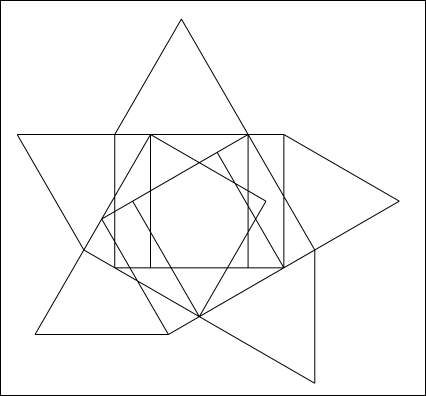
\includegraphics[width=5.0cm,trim=4 4 6 4,clip]{./images/marta/mar-3.png}
   \label{mar-3}
\end{figure}
\end{minipage} \hfill
\begin{minipage}{0.45\textwidth}
\begin{itemize}[itemsep=-3pt,parsep=2pt]
\item[] \hspace{0.5cm} FORWARD 100
\item[] \hspace{0.5cm} RIGHT 90
\item[] \hspace{0.5cm} FORWARD 100
\item[] \hspace{0.5cm} RIGHT 90
\item[] \hspace{0.5cm} FORWARD 100
\item[] \hspace{0.5cm} RIGHT 90
\item[] \hspace{0.5cm} FORWARD 100
\item[] \hspace{0.5cm} RIGHT 90
\item[] \hspace{0.5cm} FORWARD 100
\item[] \hspace{0.5cm} RIGHT 30
\item[] \hspace{0.5cm} FORWARD 100
\item[] \hspace{0.5cm} RIGHT 120
\item[] \hspace{0.5cm} FORWARD 100
\end{itemize}
\end{minipage}

\subsection{Fase IV}

Proviamo ora a cambiare la posizione finale della tartaruga e ad avviare il
programma più volte in modo tale che la casetta costruita possa non sovrapporsi
mai a quella precedente. Vediamo che cosa viene fuori!  Proviamo ad esempio ad
impostare, come ultimo comando, “RIGHT  45”.  Per svolgere questa ultima
attività, i bambini devono fare delle ipotesi e riflettere sugli angoli e sulle
ampiezze. 

Possiamo a questo punto introdurre il comando “REPEAT”, scrivendo “REPEAT”
seguito dal numero delle volte che si desidera riattivare il programma e dalle
istruzioni inserite tra parentesi quadre. Questo semplifica e rende più rapido
il procedimento, permettendo di non cliccare tutte le volte sulla voce “AVVIA
IL PROGRAMMA  LOGO” nell’apposita barra.

Che cosa sembra questa immagine? Potrebbe essere un’astronave oppure un missile
spaziale!

\begin{minipage}{0.5\textwidth}
\begin{figure}[H]
	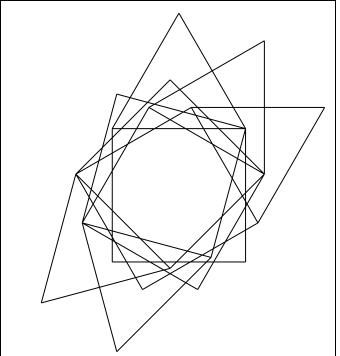
\includegraphics[width=5.0cm,trim=4 4 6 4,clip]{./images/marta/mar-4.png}
   \label{mar-4}
\end{figure}
\end{minipage} \hfill
\begin{minipage}{0.45\textwidth}
\begin{itemize}[itemsep=-3pt,parsep=2pt]
\item[] \hspace{0.5cm} REPEAT 5 [
\item[] \hspace{0.5cm} 	FORWARD 100
\item[] \hspace{0.5cm} 	RIGHT 90
\item[] \hspace{0.5cm} 	FORWARD 100
\item[] \hspace{0.5cm} 	RIGHT 90
\item[] \hspace{0.5cm} 	FORWARD 100
\item[] \hspace{0.5cm} 	RIGHT 90
\item[] \hspace{0.5cm} 	FORWARD 100
\item[] \hspace{0.5cm} 	RIGHT 90
\item[] \hspace{0.5cm} 	FORWARD 100
\item[] \hspace{0.5cm} 	RIGHT 30
\item[] \hspace{0.5cm} 	FORWARD 100
\item[] \hspace{0.5cm} 	RIGHT 120
\item[] \hspace{0.5cm} 	FORWARD 100
\item[] \hspace{0.5cm} 	RIGHT 45
\item[] \hspace{0.5cm} 	]          
\end{itemize}
\end{minipage}

E se scriviamo “RIGHT 100” come ultimo comando? Che cosa viene fuori? 

\begin{minipage}{0.5\textwidth}
\begin{figure}[H]
   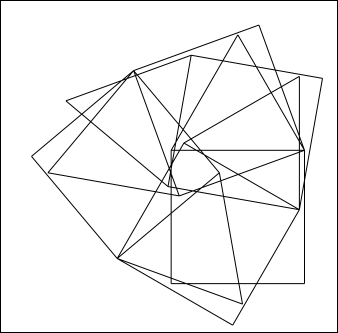
\includegraphics[width=5.0cm,trim=4 4 6 4,clip]{./images/marta/mar-5.png}
   \label{mar-5}
\end{figure}
\end{minipage} \hfill
\begin{minipage}{0.45\textwidth}
\begin{itemize}[itemsep=-3pt,parsep=2pt]
\item[] \hspace{0.5cm} REPEAT 5 [
\item[] \hspace{0.5cm} 	FORWARD 100
\item[] \hspace{0.5cm} 	RIGHT 90
\item[] \hspace{0.5cm} 	FORWARD 100
\item[] \hspace{0.5cm} 	RIGHT 90
\item[] \hspace{0.5cm} 	FORWARD 100
\item[] \hspace{0.5cm} 	RIGHT 90
\item[] \hspace{0.5cm} 	FORWARD 100
\item[] \hspace{0.5cm} 	RIGHT 90
\item[] \hspace{0.5cm} 	FORWARD 100
\item[] \hspace{0.5cm} 	RIGHT 30
\item[] \hspace{0.5cm} 	FORWARD 100
\item[] \hspace{0.5cm} 	RIGHT 120
\item[] \hspace{0.5cm} 	FORWARD 100
\item[] \hspace{0.5cm} 	RIGHT 100
\item[] \hspace{0.5cm} 	]          
\end{itemize}
\end{minipage}

E se ripetiamo per più volte ancora la serie di comandi, ad esempio per 15
volte? Che bellissimo girasole!

\begin{minipage}{0.5\textwidth}
\begin{figure}[H]
   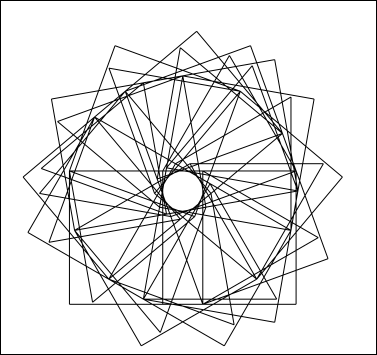
\includegraphics[width=5.0cm,trim=4 4 6 4,clip]{./images/marta/mar-6.png}
   \label{mar-6}
\end{figure}
\end{minipage} \hfill
\begin{minipage}{0.45\textwidth}
\begin{itemize}[itemsep=-3pt,parsep=2pt]
\item[] \hspace{0.5cm} REPEAT 15 [
\item[] \hspace{0.5cm} 	FORWARD 100
\item[] \hspace{0.5cm} 	RIGHT 90
\item[] \hspace{0.5cm} 	FORWARD 100
\item[] \hspace{0.5cm} 	RIGHT 90
\item[] \hspace{0.5cm} 	FORWARD 100
\item[] \hspace{0.5cm} 	RIGHT 90
\item[] \hspace{0.5cm} 	FORWARD 100
\item[] \hspace{0.5cm} 	RIGHT 90
\item[] \hspace{0.5cm} 	FORWARD 100
\item[] \hspace{0.5cm} 	RIGHT 30
\item[] \hspace{0.5cm} 	FORWARD 100
\item[] \hspace{0.5cm} 	RIGHT 120
\item[] \hspace{0.5cm} 	FORWARD 100
\item[] \hspace{0.5cm} 	RIGHT 100
\item[] \hspace{0.5cm} 	]          
\end{itemize}
\end{minipage}

Proviamo a ripeterla invece per 100 volte!! Ai bambini “strafare”, esagerare,
sperimentare “all’infinito” piacerà moltissimo! Ed ecco un sole splendente…
oppure una margherita profumata!

\begin{minipage}{0.5\textwidth}
\begin{figure}[H]
   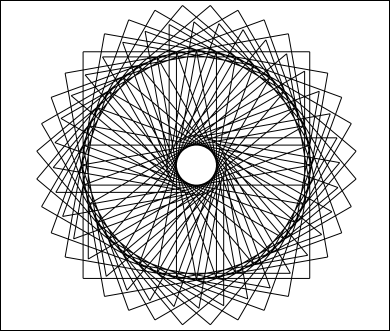
\includegraphics[width=5.0cm,trim=4 4 6 4,clip]{./images/marta/mar-7.png}
   \label{mar-7}
\end{figure}
\end{minipage} \hfill
\begin{minipage}{0.45\textwidth}
\begin{itemize}[itemsep=-3pt,parsep=2pt]
 
\item[] \hspace{0.5cm} REPEAT 100 [
\item[] \hspace{0.5cm} 	FORWARD 100
\item[] \hspace{0.5cm} 	RIGHT 90
\item[] \hspace{0.5cm} 	FORWARD 100
\item[] \hspace{0.5cm} 	RIGHT 90
\item[] \hspace{0.5cm} 	FORWARD 100
\item[] \hspace{0.5cm} 	RIGHT 90
\item[] \hspace{0.5cm} 	FORWARD 100
\item[] \hspace{0.5cm} 	RIGHT 90
\item[] \hspace{0.5cm} 	FORWARD 100
\item[] \hspace{0.5cm} 	RIGHT 30
\item[] \hspace{0.5cm} 	FORWARD 100
\item[] \hspace{0.5cm} 	RIGHT 120
\item[] \hspace{0.5cm} 	FORWARD 100
\item[] \hspace{0.5cm} 	RIGHT 100
\item[] \hspace{0.5cm}  ]
\end{itemize}          	          
\end{minipage}

Ecco cosa viene fuori invece se l’ultimo comando è “RIGHT 130” e se il
programma viene eseguito 20 volte!

\begin{minipage}{0.5\textwidth}
\begin{figure}[H]
   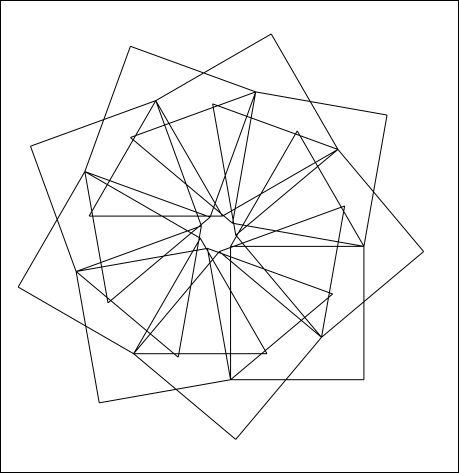
\includegraphics[width=5.0cm,trim=4 4 6 4,clip]{./images/marta/mar-8.png}
   \label{mar-8}
\end{figure}
\end{minipage} \hfill
\begin{minipage}{0.45\textwidth}
\begin{itemize}[itemsep=-3pt,parsep=2pt]
\item[] \hspace{0.5cm} REPEAT 20 [
\item[] \hspace{0.5cm} 	FORWARD 100
\item[] \hspace{0.5cm} 	RIGHT 90
\item[] \hspace{0.5cm} 	FORWARD 100
\item[] \hspace{0.5cm} 	RIGHT 90
\item[] \hspace{0.5cm} 	FORWARD 100
\item[] \hspace{0.5cm} 	RIGHT 90
\item[] \hspace{0.5cm} 	FORWARD 100
\item[] \hspace{0.5cm} 	RIGHT 90
\item[] \hspace{0.5cm} 	FORWARD 100
\item[] \hspace{0.5cm} 	RIGHT 30
\item[] \hspace{0.5cm} 	FORWARD 100
\item[] \hspace{0.5cm} 	RIGHT 120
\item[] \hspace{0.5cm} 	FORWARD 100
\item[] \hspace{0.5cm} 	RIGHT 130
\item[] \hspace{0.5cm}  ]
\end{itemize}          	          
\end{minipage}

Svolgendo questo esercizio i bambini si accorgeranno che, a partire da un certo
punto in poi, la tartaruga ripete la sequenza di movimenti senza formare una
nuova figura, ma ricominciando a creare quella precedente, sovrapposta alla
prima. Verrà spontaneo chiedersi dopo quante volte la tartaruga “ricomincia il
giro”, ossia quale è il numero di volte minimo che un determinato programma
deve essere riavviato affinché si costituisca la figura più complessa che è
possibile creare attraverso la ripetizione di quella determinata serie di
comandi. 

Prendiamo il caso di una rotazione di 90 gradi a destra rispetto alla direzione
finale della tartaruga, posizionata al termine del terzo lato del triangolo. In
questo caso la tartaruga è inclinata di 60 gradi a destra rispetto alla
verticale. Avviando il programma più volte, i bambini si accorgeranno che, fino
alla terza volta, la tartaruga costruirà una figura via via più complessa; a
partire dal quarto riavvio del programma, invece, la tartaruga comincerà a
ri-tracciare la stessa figura, sovrapponendola alla precedente.

Questo è il prodotto di tre ripetizioni di casetta, con rotazione finale di 90
gradi a destra:

\begin{minipage}{0.5\textwidth}
\begin{figure}[H]
   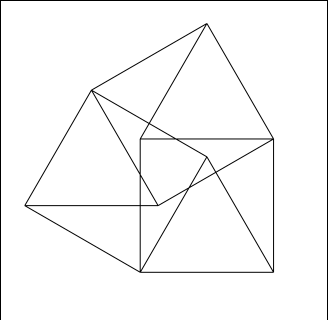
\includegraphics[width=5.0cm,trim=4 4 6 4,clip]{./images/marta/mar-9.png}
   \label{mar-9}
\end{figure}
\end{minipage} \hfill
\begin{minipage}{0.45\textwidth}
\begin{itemize}[itemsep=-3pt,parsep=2pt]
\item[] \hspace{0.5cm} REPEAT 3 [
\item[] \hspace{0.5cm} 	FORWARD 100
\item[] \hspace{0.5cm} 	RIGHT 90
\item[] \hspace{0.5cm} 	FORWARD 100
\item[] \hspace{0.5cm} 	RIGHT 90
\item[] \hspace{0.5cm} 	FORWARD 100
\item[] \hspace{0.5cm} 	RIGHT 90
\item[] \hspace{0.5cm} 	FORWARD 100
\item[] \hspace{0.5cm} 	RIGHT 90
\item[] \hspace{0.5cm} 	FORWARD 100
\item[] \hspace{0.5cm} 	RIGHT 30
\item[] \hspace{0.5cm} 	FORWARD 100
\item[] \hspace{0.5cm} 	RIGHT 120
\item[] \hspace{0.5cm} 	FORWARD 100
\item[] \hspace{0.5cm} 	RIGHT 90
\item[] \hspace{0.5cm} 	]          
\end{itemize}          	          
\end{minipage}

Questo invece è il prodotto che risulta da quattro ripetizioni della stessa
sequenza di comandi: è identico al precedente!

\begin{minipage}{0.5\textwidth}
\begin{figure}[H]
   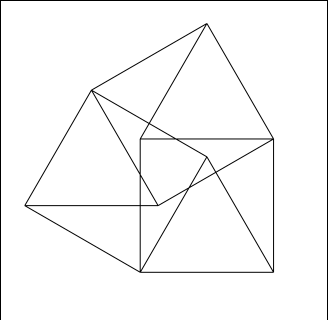
\includegraphics[width=5.0cm,trim=4 4 6 4,clip]{./images/marta/mar-9.png}
   \label{mar-10}
\end{figure}
\end{minipage} \hfill
\begin{minipage}{0.45\textwidth}
\begin{itemize}[itemsep=-3pt,parsep=2pt]
\item[] \hspace{0.5cm} REPEAT 4 [
\item[] \hspace{0.5cm} 	FORWARD 100
\item[] \hspace{0.5cm} 	RIGHT 90
\item[] \hspace{0.5cm} 	FORWARD 100
\item[] \hspace{0.5cm} 	RIGHT 90
\item[] \hspace{0.5cm} 	FORWARD 100
\item[] \hspace{0.5cm} 	RIGHT 90
\item[] \hspace{0.5cm} 	FORWARD 100
\item[] \hspace{0.5cm} 	RIGHT 90
\item[] \hspace{0.5cm} 	FORWARD 100
\item[] \hspace{0.5cm} 	RIGHT 30
\item[] \hspace{0.5cm} 	FORWARD 100
\item[] \hspace{0.5cm} 	RIGHT 120
\item[] \hspace{0.5cm} 	FORWARD 100
\item[] \hspace{0.5cm} 	RIGHT 90
\item[] \hspace{0.5cm} 	]          
\end{itemize}          	          
\end{minipage}

Tre dunque è il numero massimo di volte nelle quali si può ripetere la sequenza
di comandi così da ottenere una figura diversa, ad ogni ripetizione e, in
particolare, sempre più complessa. Proviamo a scoprire quante volte al massimo
è possibile ripetere la sequenza di comandi, per ottenere una figura sempre
diversa, nel caso in cui la rotazione finale della tartaruga, rispetto alla sua
posizione ultima, sia di 0 gradi. Questo è il caso della FASE III, nella quale
la tartaruga, alla fine della costruzione della casetta, rimane posizionata
nella direzione indicata dall’ultimo lato del triangolo-tetto, ossia inclinata
di 30 gradi a sinistra rispetto alla direzione verticale. 

In questo caso notiamo che la tartaruga esegue il programma per 12 volte prima
di ricominciare a tracciare lo stesso percorso. Anche nel caso di
un’inclinazione iniziale di 60 gradi a destra rispetto alla posizione ultima
della tartaruga, si deve avviare il programma 12 volte prima di ritrovarla
posizionata come da comando “HOME”. Se invece la facciamo ruotare di 45 gradi a
destra rispetto alla posizione ultima, si deve riavviare il programma 24 volte
prima di ritrovarla posizionata come da comando “HOME”. Notiamo che in questo
caso la tartaruga è spostata di 15 gradi a destra rispetto alla verticale.
Anche se facciamo ruotare di 15 gradi a destra rispetto alla posizione ultima,
accade la stessa cosa: si deve riavviare il programma 24 volte prima di
ritrovarla posizionata come da comando “HOME”. Notiamo che anche in questo caso
la tartaruga è spostata di 15 gradi, stavolta a sinistra, rispetto alla
verticale.

Analizzando queste corrispondenze, sembra quindi che ruotando la tartaruga,
rispetto alla posizione finale (nella direzione del terzo lato del
triangolo-tetto), di un numero di gradi n, rispetto alla verticale, sia che si
ruoti a destra sia che si ruoti a sinistra, essa dovrà ripetere il programma
uno stesso numero p di volte, prima di tornare alla posizione come da comando
“HOME”. 

Per verificare se quanto ipotizzato è vero, proviamo ad estendere questo
ragionamento anche al caso dell’inclinazione di 90 gradi a destra rispetto alla
pozione finale (caso esposto per primo, sopra). In questo caso, la tartaruga,
una volta ruotata, si ritrova inclinata di 60 gradi a destra rispetto alla
verticale. Se proviamo ad inclinarla invece di 60 gradi a sinistra, rispetto
alla stessa verticale, cosa avviene? Per farlo, dobbiamo sostituire l’ultimo
comando della serie, “RIGHT 90”, con il comando “LEFT 30”. Se il ragionamento
sopra esposto è corretto, devono risultare sufficienti 3 riavvii di programma
per far tornare la tartaruga nella posizione come da comando “HOME”. In
effetti, ciò accade: se il programma viene ripetuto quattro volte, la figura
ottenuta è la stessa che se viene ripetuto 3.

\begin{minipage}{0.5\textwidth}
\begin{figure}[H]
   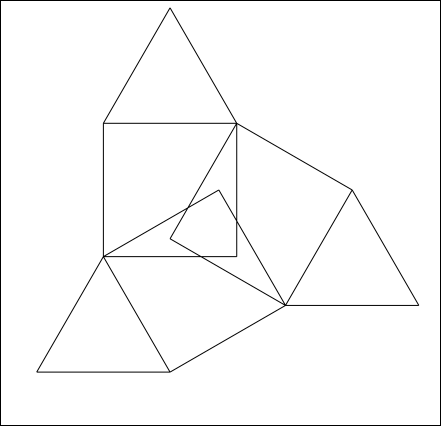
\includegraphics[width=5.0cm,trim=4 4 6 4,clip]{./images/marta/mar-10.png}
   \label{mar-11}
\end{figure}
\end{minipage} \hfill
\begin{minipage}{0.45\textwidth}
\begin{itemize}[itemsep=-3pt,parsep=2pt]
\item[] \hspace{0.5cm} REPEAT 3 [
\item[] \hspace{0.5cm} 	FORWARD 100
\item[] \hspace{0.5cm} 	RIGHT 90
\item[] \hspace{0.5cm} 	FORWARD 100
\item[] \hspace{0.5cm} 	RIGHT 90
\item[] \hspace{0.5cm} 	FORWARD 100
\item[] \hspace{0.5cm} 	RIGHT 90
\item[] \hspace{0.5cm} 	FORWARD 100
\item[] \hspace{0.5cm} 	RIGHT 90
\item[] \hspace{0.5cm} 	FORWARD 100
\item[] \hspace{0.5cm} 	RIGHT 30
\item[] \hspace{0.5cm} 	FORWARD 100
\item[] \hspace{0.5cm} 	RIGHT 120
\item[] \hspace{0.5cm} 	FORWARD 100
\item[] \hspace{0.5cm} 	LEFT 30
\item[] \hspace{0.5cm} 	]          
\end{itemize}          	          
\end{minipage}

\begin{minipage}{0.5\textwidth}
\begin{figure}[H]
   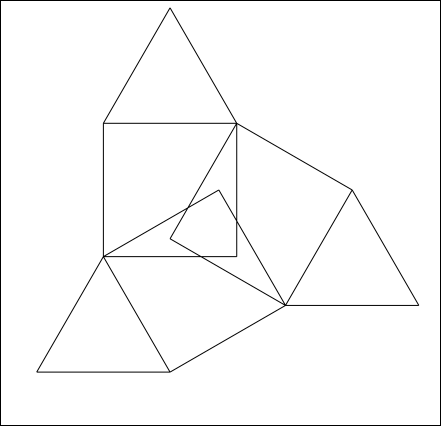
\includegraphics[width=5.0cm,trim=4 4 6 4,clip]{./images/marta/mar-10.png}
   \label{mar-12}
\end{figure}
\end{minipage} \hfill
\begin{minipage}{0.45\textwidth}
\begin{itemize}[itemsep=-3pt,parsep=2pt]
\item[] \hspace{0.5cm} REPEAT 4 [
\item[] \hspace{0.5cm} 	FORWARD 100
\item[] \hspace{0.5cm} 	RIGHT 90
\item[] \hspace{0.5cm} 	FORWARD 100
\item[] \hspace{0.5cm} 	RIGHT 90
\item[] \hspace{0.5cm} 	FORWARD 100
\item[] \hspace{0.5cm} 	RIGHT 90
\item[] \hspace{0.5cm} 	FORWARD 100
\item[] \hspace{0.5cm} 	RIGHT 90
\item[] \hspace{0.5cm} 	FORWARD 100
\item[] \hspace{0.5cm} 	RIGHT 30
\item[] \hspace{0.5cm} 	FORWARD 100
\item[] \hspace{0.5cm} 	RIGHT 120
\item[] \hspace{0.5cm} 	FORWARD 100
\item[] \hspace{0.5cm} 	LEFT 30
\item[] \hspace{0.5cm} 	]          
\end{itemize}          	          
\end{minipage}

Abbiamo dunque osservato che: 

\begin{itemize}

	\item Ruotando la tartaruga di 90 gradi a destra o di 30 gradi a
		sinistra rispetto alla posizione finale, ossia posizionandola
		inclinata di 60 gradi rispetto alla verticale, rispettivamente
		a destra o a sinistra, il numero di volte che è necessario
		riavviare il programma affinché essa torni in posizione
		iniziale “HOME” è pari a 3.
	
	\item Ruotando la tartaruga di 60 gradi a destra rispetto alla
		posizione finale oppure lasciandola in tale posizione, ossia
		posizionandola inclinata di 30 gradi rispetto alla verticale,
		rispettivamente a destra o a sinistra, il numero di volte che è
		necessario riavviare il programma affinché essa torni in
		posizione iniziale “HOME” è pari a 12.
	
	\item Ruotando la tartaruga di 45 gradi a destra o di 15 gradi a destra
		rispetto alla posizione finale, ossia posizionandola inclinata
		di 15 gradi rispetto alla verticale, rispettivamente a destra o
		a sinistra, il numero di volte che è necessario riavviare il
		programma affinché essa torni in posizione iniziale “HOME” è
		pari a 24.

\end{itemize}

A quanto pare si potrebbe continuare….

\begin{itemize}

\item Ruotando la tartaruga di 150 gradi a destra o di 90 gradi a sinistra
	rispetto alla posizione finale, ossia posizionandola inclinata di 120
		gradi rispetto alla verticale, rispettivamente a destra o a
		sinistra, il numero di volte che è necessario riavviare il
		programma affinché essa torni in posizione iniziale “HOME” è
		pari a 6.

\item Ruotando la tartaruga di 270 gradi a destra o di 210 gradi a sinistra
	rispetto alla posizione finale, ossia posizionandola inclinata di 240
		gradi rispetto alla verticale, rispettivamente a destra o a
		sinistra, il numero di volte che è necessario riavviare il
		programma affinché essa torni in posizione iniziale “HOME” è
		pari a 6.

\end{itemize}

Per tornare al nostro caso precedente, il magnifico fiore “esagerato”, ottenuto
ripetendo 100 volte la serie di comandi… Quante volte sarebbe bastato riavviare
il programma per ottenere lo stesso prodotto?

Risulta che ruotando la tartaruga di 100 gradi a destra o di 40 gradi a
sinistra rispetto alla posizione finale, ossia posizionandola inclinata di 70
gradi rispetto alla verticale, rispettivamente a destra o a sinistra, il numero
di volte che è necessario riavviare il programma affinché essa torni in
posizione iniziale “HOME” è pari a 36. Sarebbero bastate 36 volte per ottenere
la stessa figura; infatti:

\begin{minipage}{0.5\textwidth}
\begin{figure}[H]
   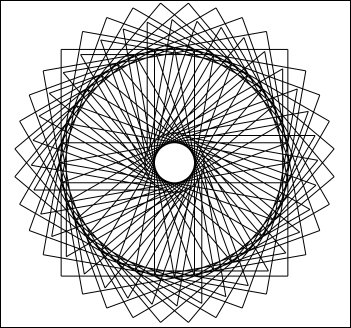
\includegraphics[width=5.0cm,trim=4 4 6 4,clip]{./images/marta/mar-11.png}
   \label{mar-13}
\end{figure}
\end{minipage} \hfill
\begin{minipage}{0.45\textwidth}
\begin{itemize}[itemsep=-3pt,parsep=2pt]
\item[] \hspace{0.5cm} REPEAT 36 [
\item[] \hspace{0.5cm} 	FORWARD 100
\item[] \hspace{0.5cm} 	RIGHT 90
\item[] \hspace{0.5cm} 	FORWARD 100
\item[] \hspace{0.5cm} 	RIGHT 90
\item[] \hspace{0.5cm} 	FORWARD 100
\item[] \hspace{0.5cm} 	RIGHT 90
\item[] \hspace{0.5cm} 	FORWARD 100
\item[] \hspace{0.5cm} 	RIGHT 90
\item[] \hspace{0.5cm} 	FORWARD 100
\item[] \hspace{0.5cm} 	RIGHT 30
\item[] \hspace{0.5cm} 	FORWARD 100
\item[] \hspace{0.5cm} 	RIGHT 120
\item[] \hspace{0.5cm} 	FORWARD 100
\item[] \hspace{0.5cm} 	RIGHT 100
\item[] \hspace{0.5cm} 	]          
\end{itemize}          	          
\end{minipage}

\begin{minipage}{0.5\textwidth}

\begin{figure}[H]
   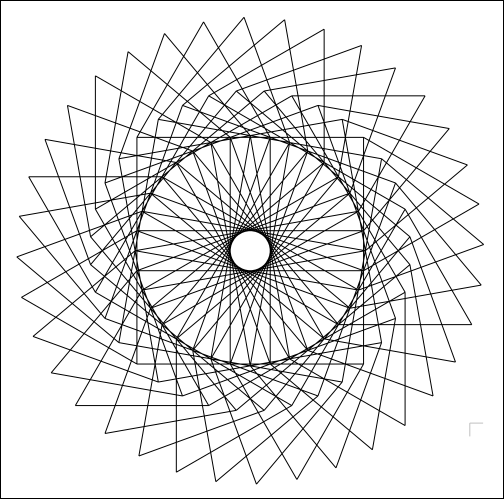
\includegraphics[width=5.0cm,trim=4 4 6 4,clip]{./images/marta/mar-12.png}
   \label{mar-14}
\end{figure}
\end{minipage} \hfill
\begin{minipage}{0.45\textwidth}
\begin{itemize}[itemsep=-3pt,parsep=2pt]
\item[] \hspace{0.5cm} REPEAT 36 [
\item[] \hspace{0.5cm} 	FORWARD 100
\item[] \hspace{0.5cm} 	RIGHT 90
\item[] \hspace{0.5cm} 	FORWARD 100
\item[] \hspace{0.5cm} 	RIGHT 90
\item[] \hspace{0.5cm} 	FORWARD 100
\item[] \hspace{0.5cm} 	RIGHT 90
\item[] \hspace{0.5cm} 	FORWARD 100
\item[] \hspace{0.5cm} 	RIGHT 90
\item[] \hspace{0.5cm} 	FORWARD 100
\item[] \hspace{0.5cm} 	RIGHT 30
\item[] \hspace{0.5cm} 	FORWARD 100
\item[] \hspace{0.5cm} 	RIGHT 120
\item[] \hspace{0.5cm} 	FORWARD 100
\item[] \hspace{0.5cm} 	LEFT 40
\item[] \hspace{0.5cm} 	]          
\end{itemize}          	          
\end{minipage}

E ancora, per tornare ai nostri “esercizi” di creatività, risulta che ruotando
la tartaruga di 130 gradi a destra o di 70 gradi a sinistra rispetto alla
posizione finale, ossia posizionandola inclinata di 100 gradi rispetto alla
verticale, rispettivamente a destra o a sinistra, il numero di volte che è
necessario riavviare il programma affinché essa torni in posizione iniziale
“HOME” è pari a 9. Sarebbero bastate 9 volte per ottenere la stessa figura;
infatti:

\begin{minipage}{0.5\textwidth}
\begin{figure}[H]
   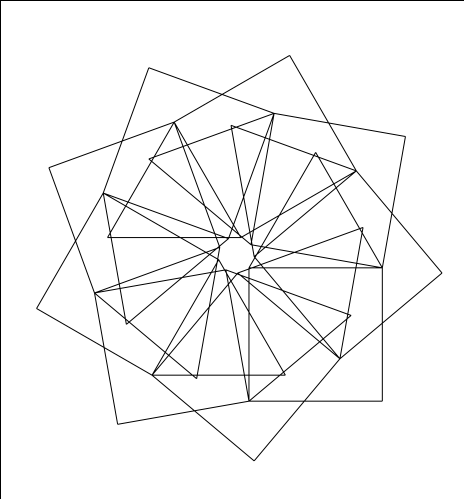
\includegraphics[width=5.0cm,trim=4 4 6 4,clip]{./images/marta/mar-13.png}
   \label{mar-15}
\end{figure}
\end{minipage} \hfill
\begin{minipage}{0.45\textwidth}
\begin{itemize}[itemsep=-3pt,parsep=2pt]
\item[] \hspace{0.5cm} REPEAT 9 [
\item[] \hspace{0.5cm} 	FORWARD 100
\item[] \hspace{0.5cm} 	RIGHT 90
\item[] \hspace{0.5cm} 	FORWARD 100
\item[] \hspace{0.5cm} 	RIGHT 90
\item[] \hspace{0.5cm} 	FORWARD 100
\item[] \hspace{0.5cm} 	RIGHT 90
\item[] \hspace{0.5cm} 	FORWARD 100
\item[] \hspace{0.5cm} 	RIGHT 90
\item[] \hspace{0.5cm} 	FORWARD 100
\item[] \hspace{0.5cm} 	RIGHT 30
\item[] \hspace{0.5cm} 	FORWARD 100
\item[] \hspace{0.5cm} 	RIGHT 120
\item[] \hspace{0.5cm} 	FORWARD 100
\item[] \hspace{0.5cm} 	RIGHT 130
\item[] \hspace{0.5cm} 	]          
\end{itemize}          	          
\end{minipage}

\begin{minipage}{0.5\textwidth}
\begin{figure}[H]
   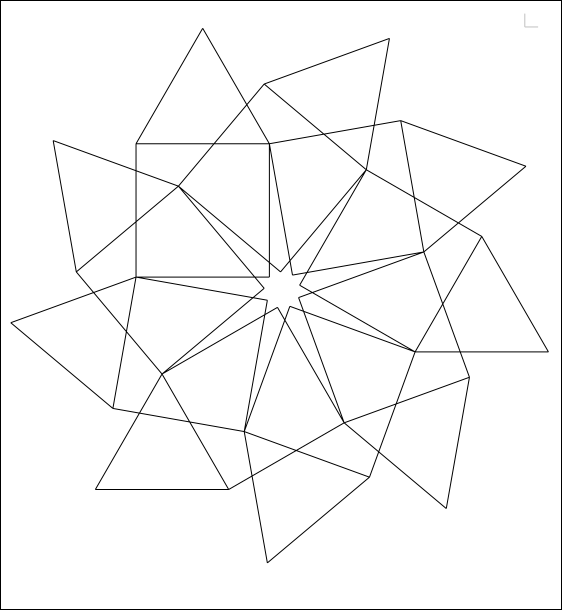
\includegraphics[width=5.0cm,trim=4 4 6 4,clip]{./images/marta/mar-14.png}
   \label{mar-16}
\end{figure}
\end{minipage} \hfill
\begin{minipage}{0.45\textwidth}
\begin{itemize}[itemsep=-3pt,parsep=2pt]
\item[] \hspace{0.5cm} REPEAT 9 [
\item[] \hspace{0.5cm} 	FORWARD 100
\item[] \hspace{0.5cm} 	RIGHT 90
\item[] \hspace{0.5cm} 	FORWARD 100
\item[] \hspace{0.5cm} 	RIGHT 90
\item[] \hspace{0.5cm} 	FORWARD 100
\item[] \hspace{0.5cm} 	RIGHT 90
\item[] \hspace{0.5cm} 	FORWARD 100
\item[] \hspace{0.5cm} 	RIGHT 90
\item[] \hspace{0.5cm} 	FORWARD 100
\item[] \hspace{0.5cm} 	RIGHT 30
\item[] \hspace{0.5cm} 	FORWARD 100
\item[] \hspace{0.5cm} 	RIGHT 120
\item[] \hspace{0.5cm} 	FORWARD 100
\item[] \hspace{0.5cm} 	RIGHT 70
\item[] \hspace{0.5cm} 	]          
\end{itemize}          	          
\end{minipage}

\vskip 1cm

Insomma, sembra che la direzione di rotazione della tartaruga rispetto alla
posizione finale, incida fortemente sull’immagine che si potrà ottenere ad
un’eventuale ripetizione del programma,  ma che, a patto che essa sia di un
numero sempre uguale di gradi, sia che venga effettuata a destra sia che venga
effettuata a sinistra rispetto alla verticale, il numero di volte necessario
affinché la tartaruga torni alla posizione “HOME” rimane invariato.

Viene ora da domandarsi se sia possibile procedere verso un’ulteriore
generalizzazione, a partire dai dati raccolti e dalle osservazioni fatte.  In
particolare, ci si chiede se esista una qualche relazione matematica tra il
numero di gradi di inclinazione della tartaruga rispetto alla verticale in
posizione finale (ossia dopo aver costruito la casetta) e il numero di volte
che essa deve rieseguire il programma per poter tornare alla posizione “HOME”.

Raccogliamo i dati in una tabella:

\begin{center}
\begin{tabular}{| >{\centering\arraybackslash}m{1in} | >{\centering\arraybackslash}m{1in} |}
\hline
Gradi rotazione rispetto alla verticale & Numero di volte che il programma deve riavviarsi per tornare a posizione "home" \\ \hline
\hspace{3pt}  15  &     24   \\ \hline 
\hspace{3pt}  30  &     12   \\ \hline 
\hspace{3pt}  60  & \hspace{2pt}     3   \\ \hline 
\hspace{3pt}  70  &     36   \\ \hline 
 100  & \hspace{2pt}     9   \\ \hline 
 120  & \hspace{2pt}   6   \\ \hline 
 240  & \hspace{2pt}    6 \\ \hline 
\end{tabular}
\end{center}

Purtroppo non sembra emergere alcuna relazione…. E qui il pensiero si sofferma e prende respiro...
Forse potremmo fare altre ipotesi?

\vskip 0.3cm

Marta


\subsection{Una prima soluzione}


Probabilmente si potrebbe procedere a individuare una risposta matematica
generale al quesito di Marta, ovvero formulare una descrizione teorica la
quale, partendo da precisi e esaustivi presupposti, consenta di individuare una
risposta corretta per tutti casi. Non disponendo del tempo per affrontare la
questione in tali termini, ci venne a suo tempo naturale procedere per via
euristica, esplorando una quantità di casi particolari. È emerso subito un
primo fatto: in molti casi, il numero di ripetizioni minimo $N$ viene dato
correttamente da questa relazione:

\begin{equation}
N=\frac{360}{\theta \bmod 60}
\end{equation} 

dove $\theta$ è l'angolo di inclinazione della tartaruga rispetto alla
verticale in posizione finale e $\bmod$ è l'operazione "modulo", che dà il
resto della divisione fra i due operandi: se, per esempio, $\theta=365$ allora
$\theta \bmod 60 = 5$. Tuttavia, insistendo si scopre altrettanto presto che vi
sono valori particolari di $\theta$, che costituiscono casi che potremmo
definire degenerati, nei quali il numero di ripetizioni viene sorprendentemente
piccolo. Facendo prove di questo genere, giungemmo alla seguente espressione:

\begin{equation} \label{eq:1}
N=
\begin{cases}
\begin{cases}
3, & \text{per } \theta/60=1 \\
6, & \text{per } \theta/60 \ne 1
\end{cases}, & \text{per } \theta \bmod 60 = 0  \\
\frac{360}{\theta \bmod 60}, & \text{per } \theta \bmod 60 \neq 0
\end{cases}
\end{equation}

Poiché questa relazione consentiva di rispondere a tutti i casi elencati nella
tabella proposta da Marta ci ritenemmo soddisfatti, ben consapevoli tuttavia,
che non era affatto detto che la soluzione trovata fosse esaustiva per tutti i
casi possibili. Ci accontentammo quindi dei risultati forniti dal codice Logo
che esprime la suddetta formula, dove la variabile T rappresenta $\theta$ e
NVOLTE rappresenta $N$:

\vskip 1cm

\begin{minipage}{1.0\textwidth}
\begin{itemize}[itemsep=-3pt,parsep=2pt]
\item[] \hspace{0.5cm}  1\hspace{8pt}TO NVOLTE T
\item[] \hspace{0.5cm}  2\hspace{8pt}\hspace{8pt}T = ABS(T)
\item[] \hspace{0.5cm}	3\hspace{8pt}\hspace{8pt}R = T \% 60
\item[] \hspace{0.5cm}  4\hspace{8pt}\hspace{8pt}IF R = 0 [ IF T /60 = 1 [ N = 3 ] [ N = 6 ] ] [ N = 360/R ]
\item[] \hspace{0.5cm}  5\hspace{8pt}\hspace{8pt}OUTPUT N
\item[] \hspace{0.5cm}  7\hspace{8pt}END
\item[] \hspace{0.5cm}  8
\item[] \hspace{0.5cm}  9\hspace{8pt}TO CASA
\item[] \hspace{0.3cm} 10\hspace{8pt}FORWARD 100 
\item[] \hspace{0.3cm} 11\hspace{8pt}RIGHT 90 
\item[] \hspace{0.3cm} 12\hspace{8pt}FORWARD 100 
\item[] \hspace{0.3cm} 13\hspace{8pt}RIGHT 90 
\item[] \hspace{0.3cm} 14\hspace{8pt}FORWARD 100 
\item[] \hspace{0.3cm} 15\hspace{8pt}RIGHT 90 
\item[] \hspace{0.3cm} 16\hspace{8pt}FORWARD 100 
\item[] \hspace{0.3cm} 17\hspace{8pt}RIGHT 90 
\item[] \hspace{0.3cm} 18\hspace{8pt}FORWARD 100 
\item[] \hspace{0.3cm} 19\hspace{8pt}RIGHT 30 
\item[] \hspace{0.3cm} 20\hspace{8pt}FORWARD 100 
\item[] \hspace{0.3cm} 21\hspace{8pt}RIGHT 120 
\item[] \hspace{0.3cm} 22\hspace{8pt}FORWARD 100 
\item[] \hspace{0.3cm} 23 END
\item[] \hspace{0.3cm} 24
\item[] \hspace{0.3cm} 25 TO FIGURA NV TETA
\item[] \hspace{0.3cm} 26\hspace{8pt}REPEAT NV [ 
\item[] \hspace{0.3cm} 27\hspace{8pt}CASA
\item[] \hspace{0.3cm} 28\hspace{8pt}RIGHT TETA+30
\item[] \hspace{0.3cm} 29    ]
\item[] \hspace{0.3cm} 30 END
\item[] \hspace{0.3cm} 31
\item[] \hspace{0.3cm} 32 TO FIG TETA
\item[] \hspace{0.3cm} 33\hspace{8pt}CLEARSCREEN
\item[] \hspace{0.3cm} 34\hspace{8pt}NV = NVOLTE TETA
\item[] \hspace{0.3cm} 35\hspace{8pt}PRINT NV
\item[] \hspace{0.3cm} 36\hspace{8pt}FIGURA NV TETA
\item[] \hspace{0.3cm} 37 END
\item[] \hspace{0.3cm} 38
\item[] \hspace{0.3cm} 39 CLEARSCREEN
\item[] \hspace{0.3cm} 40 HOME
\item[] \hspace{0.3cm} 41 HIDETURTLE
\item[] \hspace{0.3cm} 42
\item[] \hspace{0.3cm} 43 T = -5
\item[] \hspace{0.3cm} 44 FIG T                                                              
\end{itemize}          	          
\end{minipage}

\vskip 1cm

\section{L'alternativa di Alberto} \label{se:altenativa-alberto}

Successivamente è capitato di riproporre la riflessione di Marta nel corso di
perfezionamento "Le competenze digitali nella scuola". Uno dei partecipanti,
Alberto Averono, insegnante di informatica presso un istituto tecnico, ha
rilanciato la questione, proponendo un diverso modo di codificare il problema:

\begin{quote} Buongiorno, siccome il racconto del viaggio di Marta ha stimolato
	la mia curiosità, durante la narrazione di martedì sera ho avuto due
	idee:

	\begin{itemize}

		\item se la Tartaruga ci dicesse quante case disegna prima di
			ritrovarsi a casa senza dover fare calcoli?

		\item se la Tartaruga fosse ricorsiva, consentendoci così di
	semplificare il codice?  \end{itemize}

\end{quote}

E questo è il codice alternativo proposto da Alberto:  

\vskip 1cm

\begin{minipage}{1.0\textwidth}
\begin{itemize}[itemsep=-3pt,parsep=2pt]
\item[] \hspace{0.5cm}  1\hspace{8pt}TO CASA T NV PORIG 
\item[] \hspace{0.5cm}  2\hspace{8pt}\hspace{8pt}PCORR = POSITION
\item[] \hspace{0.5cm}	3\hspace{8pt}\hspace{8pt}IF PCORR = PORIG  AND NOT NV = 0 [ PRINT NV STOP ] 
\item[] \hspace{0.5cm}  4\hspace{8pt}\hspace{8pt}FORWARD 100 
\item[] \hspace{0.5cm}  5\hspace{8pt}\hspace{8pt}RIGHT 90 
\item[] \hspace{0.5cm}  7\hspace{8pt}\hspace{8pt}FORWARD 100 
\item[] \hspace{0.5cm}  8\hspace{8pt}\hspace{8pt}RIGHT 90 
\item[] \hspace{0.5cm}  9\hspace{8pt}\hspace{8pt}FORWARD 100 
\item[] \hspace{0.3cm} 10\hspace{8pt}\hspace{8pt}RIGHT 90 
\item[] \hspace{0.3cm} 11\hspace{8pt}\hspace{8pt}FORWARD 100 
\item[] \hspace{0.3cm} 12\hspace{8pt}\hspace{8pt}RIGHT 90 
\item[] \hspace{0.3cm} 13\hspace{8pt}\hspace{8pt}FORWARD 100 
\item[] \hspace{0.3cm} 14\hspace{8pt}\hspace{8pt}RIGHT 30 
\item[] \hspace{0.3cm} 15\hspace{8pt}\hspace{8pt}FORWARD 100 
\item[] \hspace{0.3cm} 16\hspace{8pt}\hspace{8pt}RIGHT 120 
\item[] \hspace{0.3cm} 17\hspace{8pt}\hspace{8pt}FORWARD 100
\item[] \hspace{0.3cm} 18\hspace{8pt}\hspace{8pt}RIGHT T + 30
\item[] \hspace{0.3cm} 19\hspace{8pt}\hspace{8pt}NV = NV + 1
\item[] \hspace{0.3cm} 20\hspace{8pt}\hspace{8pt}CASA T NV P1                                   
\item[] \hspace{0.3cm} 21\hspace{8pt}END
\item[] \hspace{0.3cm} 22\hspace{8pt}
\item[] \hspace{0.3cm} 23\hspace{8pt}CLEARSCREEN   
\item[] \hspace{0.3cm} 24\hspace{8pt}HOME
\item[] \hspace{0.3cm} 25\hspace{8pt}P = POSITION
\item[] \hspace{0.3cm} 26\hspace{8pt}HIDETURTLE
\item[] \hspace{0.3cm} 27\hspace{8pt}CASA 30 0 PORIG  
\end{itemize}          	          
\end{minipage}

\vskip 1cm

In questo codice la casa viene disegnata con una procedura che necessita di tre
argomenti: T che rappresenta l'angolo $\theta$ di inclinazione della tartaruga
rispetto alla verticale in posizione finale, NV è il numero di volte che si
deve rieseguire il codice per poter tornare alla posizione “HOME” e PORIG contiene
la posizione inziale della Tartaruga.

Conclude Alberto:  

\begin{quote}
Supposto che il codice sia corretto, direi che
\begin{enumerate}
	\item la Tartaruga termina di costruire una casa nel punto HOME solo
		per angoli multipli di 30,
	\item se l’angolo è 180 non torna mai,
	\item per gli angoli 270 e 300 disegna 4 case e 3 case
		contro le 12 e 6 previste rispettivamente dalla formula
		\ref{eq:1},
	\item per tutti gli altri angoli multipli di 30 i risultati coincidono,
	\item con angoli non multipli di 30 ripete il disegno ma non termina
		una casa esattamente nel punto HOME per cui non si può
		utilizzare in quei casi (a meno di modifiche). 
\end{enumerate}
\end{quote}  
  
È interessante entrare nel dettaglio delle proposte di Alberto perché questo ci
consente di fare alcune importanti considerazioni, non solo relativamente al
coding ma anche a fatti prettamente matematici. 

La prima proposta è quella di lasciare che la Tartaruga "riconosca" da sola la
posizione da cui era partita. Messa in questi termini, viene in effetti da
domandarsi perché confondersi con formule arzigogolate quando è possibile
affidare tutto al calcolo numerico? Benissimo: accettiamo per il momento questa
proposta, che nel codice di Alberto si realizza nell'istruzione 3, dove si
controlla se la posizione corrente, PCORR, è eguale alla posizione originale,
PORIG. Il controllo viene fatto a meno che non si tratti della prima iterazione
(NV=0), per la quale è ovvio che le due condizioni coincidono. Se così non è
(NV$\ne$0) e se si verifica che la Tartaruga sia tornata alla posizione
originale (PCORR=PORIG) allora il programma stampa il valore NV dell'iterazione
corrente e si ferma (STOP).

La seconda proposta consiste nel sostituire il ciclo di ripetizioni usato da
Marta con una procedura ricorsiva. Alberto realizza questo mediante
l'istruzione 20, dove la procedura CASA chiama se stessa ripassando gli stessi
parametri che aveva ricevuto a sua volta. È un'ottima applicazione del
costrutto ricorsivo che avevamo descritto nel capitolo \ref{cap:magia-specchi}.

Passiamo ora a commentare i risultati, così come sono stati riassunti da Alberto.

\begin{enumerate}
	\item \label{it:1} \textit{La Tartaruga termina di costruire una casa nel punto HOME solo
		per angoli multipli di 30}. Come dire che la Tartaruga non
		riconosce sempre bene la propria posizione di origine. Questo
		è effettivamente un problema molto interessante che discutiamo
		in in dettaglio successivamente.
	\item \textit{Se l’angolo è 180 non torna mai}. Vero. È un caso particolare che
		ci era sfuggito. Possiamo dire che per $\theta=180$ il processo
		diverge. Lo aggiungiamo alla formula \ref{eq:1}.
	\item \textit{Per gli angoli 270 e 300 disegna 4 case e 3 case
		contro le 12 e 6 previste rispettivamente dalla formula
		\ref{eq:1}}. Vero anche questo. Si tratta di altri casi
		"degeneri" che andiamo ad aggiungere agli altri.
	\item \textit{Per tutti gli altri angoli multipli di 30 i risultati coincidono}.
		Sì, ma non sempre, come vediamo fra poco.
	\item \textit{Con angoli non multipli di 30 ripete il disegno ma non termina
		una casa esattamente nel punto HOME per cui non si può
		utilizzare in quei casi (a meno di modifiche)}. E questo è il
		problema menzionato al punto \ref{it:1}.
\end{enumerate}
  
Per iniziare facciamo la cernita dei casi particolari, cercando le regolarità.
Vediamo i primi 31, partendo da $\theta = 0$:

\begin{center}
\begin{tabular}{| >{\centering\arraybackslash}m{1in} | >{\centering\arraybackslash}m{1in} |}
\hline
Gradi di rotazione rispetto alla verticale & Numero di volte che il programma deve riavviarsi per tornare a posizione "home" \\ \hline
\hspace{3pt}\hspace{3pt}   0  & \hspace{2pt}     2   \\ \hline 
\hspace{3pt}  30  &     12   \\ \hline 
\hspace{3pt}  60  & \hspace{2pt}     3   \\ \hline 
\hspace{3pt}  90  & \hspace{2pt}     4   \\ \hline 
 120  & \hspace{2pt}     6   \\ \hline 
 150  &     12   \\ \hline 
 180  & $\infty$ \\ \hline 
 210  &     12   \\ \hline
 240  & \hspace{2pt}     6   \\ \hline
 270  & \hspace{2pt}     4   \\ \hline
 300  & \hspace{2pt}     3   \\ \hline
 330  &     12   \\ \hline
 360  & \hspace{2pt}     2   \\ \hline
 390  &     12   \\ \hline
 420  & \hspace{2pt}     3   \\ \hline
 450  & \hspace{2pt}     4   \\ \hline
 480  & \hspace{2pt}     6   \\ \hline
 510  &     12   \\ \hline
 540  & $\infty$ \\ \hline 
 570  &     12   \\ \hline
 600  & \hspace{2pt}     6   \\ \hline
 630  & \hspace{2pt}     4   \\ \hline
 660  & \hspace{2pt}     3   \\ \hline
 690  &     12   \\ \hline
 720  & \hspace{2pt}     2   \\ \hline
 750  &     12   \\ \hline
 780  & \hspace{2pt}     3   \\ \hline
 810  & \hspace{2pt}     4   \\ \hline
 840  & \hspace{2pt}     6   \\ \hline
 870  &     12   \\ \hline
 900  & $\infty$ \\ \hline
\end{tabular}
\end{center}
 
Se proviamo a descrivere in linguaggio matematico le regolarità che vediamo in
questa tabella otteniamo la seguente espressione, abbastanza più complicata
della precedente (\ref{eq:1}):

\begin{equation} \label{eq:2}
N=
\begin{cases}
   \begin{cases}
      2, \text{per } \theta/30 \in \{(n-1) \times 360\} \\
      3, \begin{cases}
            \text{per } \theta/30 \in \{60+(n-1) \times 360\}  \\
            \text{per } \theta/30 \in \{300+(n-1) \times 360\} \\
         \end{cases} \\
      4, \begin{cases}
            \text{per } \theta/30 \in \{90+(n-1) \times 360\}  \\
            \text{per } \theta/30 \in \{270+(n-1) \times 360\} \\
         \end{cases} \\
      6, \begin{cases}
            \text{per } \theta/30 \in \{120+(n-1) \times 360\}  \\
            \text{per } \theta/30 \in \{240+(n-1) \times 360\} \\
         \end{cases} \\
      12,\begin{cases}
            \text{per } \theta/30 \in \{150+(n-1) \times 360\}  \\
            \text{per } \theta/30 \in \{210+(n-1) \times 360\} \\
         \end{cases} \\
      \infty, \text{per } \theta/30 \in \{180+n \times 360\} \\
   \end{cases}, & \text{per } \theta \bmod 30 = 0  \\
%   \frac{360}{\theta \bmod 30}, & \text{per } \theta \bmod 30 \ne 0
   360/(\theta \bmod 30), & \text{per } \theta \bmod 30 \ne 0
\end{cases}
\end{equation}

dove $n \in \{1,2,\dots\}$.

Non è difficile tradurre in codice LibreLogo questo schema, analogamente a
quanto avevamo fatto nella versione più semplice, e questa sarebbe la via che
avevamo proposto in origine. Alberto proponeva invece altro, ovvero di far
"riconoscere" alla tartaruga medesima la posizione originale, qualora ci si
ritrovasse dopo un certo numero di ripetizioni, e quello sarebbe il numero
cercato.

La proposta è interessante, diciamo che è più di sapore numerico che
matematico. La soluzione più prettamente matematica è la precedente, dove con
il ragionamento cerchiamo una regola generale che solo alla fine applichiamo
numericamente. La proposta di Alberto è invece numerica perché si affida al
confronto fra numeri calcolati. Non esiste un criterio assoluto per stabilire
quale sia il metodo migliore, dipende dal contesto.

Qui tuttavia è Alberto stesso che segnala un problema, ovvero che la Tartaruga
termina di costruire una casa nel punto HOME solo per angoli $\theta = 30$.
Perché succede questo? Prima di rispondere dobbiamo aggiungere un'altra
complicazione. Cercando di riprodurre i risultati ottenuti da Alberto, mi sono
accorto che in realtà la Tartaruga può perdersi anche in altri casi, anche quando
$\theta$ è un multiplo di 30 gradi, e questo comportamento dipende addirittura
dal computer che ospita la Tartaruga! Ma come è possibile una cosa del genere?
Come può la Tartaruga, che è pur sempre una creatura determinata da un software
che viene eseguito in una macchina apparentemente perfettamente determinata,
stupidamente meccanica nei comportamenti, come il computer, comportarsi invece
come una creatura bizzosa, che decide come contenersi a seconda delle
circostanze? E di quali circostanze? Era già strano che le cose funzionassero
solo per valori di $\theta$ multipli di 30 gradi, ma mettersi a fare le bizze
anche per questi e su un computer sì e su un altro no è troppo! Eppure è quello
che succede ed è una fortuna per noi perché ci consente di sbirciare meglio in
un aspetto illuminante riguardo alla relazione fra matematica e \textit{computer
science}. In buona parte dell'opinione comune, tutte le scienze classiche e
tecnologiche ricadono in un ambito dominato dall'esattezza e da una sorta di
meccanicità. Questa visione genera in molti il concetto che il coding sia un
qualcosa di automatico, fatto di pratiche rigidamente predeterminate che si
riducono ad una sorta di "simulazione" di robot. È un'idea profondamente
sbagliata, generata dall'ignoranza delle questioni pertinenti.

Vediamo come stanno le cose nel nostro problema. Nel momento in cui scrivo
dispongo di tre computer diversi e scopro che... la Tartaruga si comporta
diversamente su ciascuno di essi. Prendiamo il caso $\theta=30$ gradi:

% https://tex.stackexchange.com/questions/2441/how-to-add-a-forced-line-break-inside-a-table-cell
\begin{table}[H] \label{tab:computer}
\begin{center}
\begin{tabular}{| c | c | c |}
\hline
\thead{Computer} & \thead{Versione di \\ Ubuntu} & \thead[l]{Numero di volte che \\ il programma deve riavviarsi \\ per tornare  a posizione "home"} \\
\hline
\makecell[l]{Laptop Lenovo Thinkpad X220 \\ Intel Core i5-2520M 2.50GHz \\ Ubuntu 16.04 \\ 32 bit} & 5.2.7.2 & 3 \\
\hline 
\makecell[l]{Laptop Lenovo Thinkpad X220 \\ Intel Core i7-2640M 2.80GHz \\ Windows 7 \\ 64 bit} & 5.1.2.2 & $\infty$ \\
\hline 
\makecell[l]{Minitower Acer Aspire XC100 \\ AMD E1-1500 1.50GHz \\ Ubuntu 16.04 \\ 64 bit} & 5.1.6.2 & 6 \\
\hline 
\end{tabular}
\end{center}
\end{table}

Eppure il codice eseguito è identico. Come può accadere una cosa simile? Una
delle prime cose che un collaboratore più grande mi insegnò, quando venni
in contatto con il primo computer (nel 1977), fu: quando non capisci cosa
succede fai stampare al computer tutti i dati intermedi\footnote{Qualcuno si
domanderà come si possono produrre le tabelle sottostanti con LibreLogo, che
sembra tutto orientato alla grafica. Il fatto è che LibreLogo è scritto nel
linguaggio Python, derivandone tutta una serie di caratteristiche, non
esplicitate nel manuale di LibreLogo. Fra queste capacità "clandestine" c'è
anche quella di poter leggere il contenuto di file, crearli e scriverci dentro.
Dedicheremo un'appendice a queste possibilità.}. Vediamo quindi il caso del
laptop Ubuntu, considerando la sequenza delle posizioni PCORR raggiunte dalla
Tartaruga alla fine del disegno di ogni casa, confrontate con la posizione
originale, PORIG. Occorre tenere presente che dire posizione significa dire due
numeri, ovvero le coordinate X e Y nella pagina, per cui ad esempio PORIG =
[297.41102362204725, 420.71811023622047], secondo le convenzioni descritte
nella sezione \ref{se:spazio-pagina}.

% https://tex.stackexchange.com/questions/9485/how-to-fix-table-position
\begin{table}[H]
\begin{center}
\begin{tabular}{| c | c | c |}
\hline
	NV & PCORR[0] (la X) & PORIG[0] (la X) \\ \hline
0 & 297.41102362204725 & 297.41102362204725 \\ \hline
1 & 347.41417322834644 & 297.41102362204725 \\ \hline
2 & 279.0992125984252 & 297.41102362204725 \\ \hline
\colorbox{yellow}{3} & \colorbox{yellow}{297.41102362204725} & \colorbox{yellow}{297.41102362204725} \\
\hline
\end{tabular}
\caption{Coordinate X delle posizioni correnti PCORR e della posizione originale PORIG con il laptop Ubuntu. La posizione viene ritrovata correttamente dopo la terza ripetizione. NV è il numero di volte che il programma deve riavviarsi per tornare a posizione "home", PCORR è la posizione corrente della Tartaruga e PORIG la posizione iniziale. Le variabili PCORR e PORIG sono costituite da coppie di numeri che sono le coordinate della Tartaruga nello spazio della pagina.}
\end{center}
\end{table}

\begin{table}[H]
\begin{center}
\begin{tabular}{| c | c | c |}
\hline
	NV & PCORR[1] (la Y) & PORIG[1] (la Y) \\ \hline
0 & 420.71811023622047 & 420.71811023622047 \\ \hline
1 & 370.7149606299212 & 420.71811023622047 \\ \hline
2 & 352.4031496062992 & 420.71811023622047 \\ \hline
\colorbox{yellow}{3} & \colorbox{yellow}{420.71811023622047} & \colorbox{yellow}{420.71811023622047} \\
\hline
\end{tabular}
\caption{Coordinate Y delle posizioni coorrenti PCORR e della posizione originale PORIG con il laptop Ubuntu.}
\end{center}
\end{table}

Qui vediamo che la Tartaruga conferma la congettura di Alberto: il disegno
consiste in tre casette incastrate e la Tartaruga si ferma diligentemente alla
fine della terza ripetizione. In giallo è evidenziata la perfetta
corrispondenza fra la posizione corrente PCORR alla terza ripetizione e la
posizione originale PORIG (le X e le Y sono identiche).

Vediamo ora cosa succede girando lo stesso codice nel portatile con Windows.

% https://it.sharelatex.com/learn/Using_colours_in_LaTeX
% http://www.pirbot.com/mirrors/ctan/macros/latex/required/graphics/color.pdf
\begin{table}[H]

\begin{center}
\begin{tabular}{| c | c | c |}
\hline
	NV & PCORR[0] (la X) & PORIG[0] (la X) \\ \hline
\hline
0 & 297.46771653543306 & 297.4393700787401 \\ \hline
1 & 347.47086614173224 & 297.4393700787401 \\ \hline
2 & 279.18425196850393 & 297.4393700787401 \\ \hline
\colorbox{magenta}{3} & \colorbox{yellow}{297.4}\colorbox{magenta}{96062992126} & \colorbox{yellow}{297.4}\colorbox{magenta}{393700787401} \\ \hline
4 & 347.4992125984252 & 297.4393700787401 \\ \hline
5 & 279.21259842519686 & 297.4393700787401 \\ \hline
\colorbox{magenta}{6} & \colorbox{yellow}{297.4}\colorbox{magenta}{96062992126} & \colorbox{yellow}{297.4}\colorbox{magenta}{393700787401} \\ \hline
7 & 347.4992125984252 & 297.4393700787401 \\ \hline
\colorbox{yellow}{$\infty$} & \colorbox{yellow}{$\cdots$} & \colorbox{yellow}{$\cdots$} \\
\hline
% 9 & [297.496062992126, 420.71811023622047] & [297.4393700787401, 420.6897637795276] \\
% \hline
% 10 & [347.4992125984252, 370.68661417322835] & [297.4393700787401, 420.6897637795276] \\
% \hline
% 11 & [279.21259842519686, 352.4031496062992] & [297.4393700787401, 420.6897637795276] \\
% \hline
% 12 & [297.496062992126, 420.71811023622047] & [297.4393700787401, 420.6897637795276] \\
% \hline
% 13 & [347.4992125984252, 370.68661417322835] & [297.4393700787401, 420.6897637795276] \\
% \hline
% 14 & [279.21259842519686, 352.4031496062992] & [297.4393700787401, 420.6897637795276] \\
% \hline
\end{tabular}
\caption{Coordinate X delle posizioni correnti PCORR e della posizione originale PORIG con il laptop Windows. La posizione non viene mai ritrovata correttamente - perlomeno per le prime cento ripetizioni che sono state lasciate fare alla macchina. Sono evidenziate in magenta le ripetizioni dove la Tartaruga ci va vicino.}
\end{center}
\end{table}

\begin{table}[H]

\begin{center}
\begin{tabular}{| c | c | c |}
\hline
	NV & PCORR[1] (la Y) & PORIG[1] (la Y) \\ \hline
\hline
0 & 420.71811023622047 & 420.6897637795276 \\ \hline
1 & 370.68661417322835 & 420.6897637795276 \\ \hline
2 & 352.4031496062992 & 420.6897637795276 \\ \hline
\colorbox{magenta}{3} & \colorbox{yellow}{420.}\colorbox{magenta}{71811023622047} & \colorbox{yellow}{420.}\colorbox{magenta}{6897637795276} \\ \hline
4 & 370.7149606299212 & 420.6897637795276 \\ \hline
5 & 352.4031496062992 & 420.6897637795276 \\ \hline
\colorbox{magenta}{6} & \colorbox{yellow}{420.}\colorbox{magenta}{71811023622047} & \colorbox{yellow}{420.}\colorbox{magenta}{6897637795276} \\ \hline
7 & 370.7149606299212 & 420.6897637795276 \\ \hline
\colorbox{yellow}{$\infty$} & \colorbox{yellow}{$\cdots$} & \colorbox{yellow}{$\cdots$} \\
\hline
% 9 & [297.496062992126, 420.71811023622047] & [297.4393700787401, 420.6897637795276] \\
% \hline
% 10 & [347.4992125984252, 370.68661417322835] & [297.4393700787401, 420.6897637795276] \\
% \hline
% 11 & [279.21259842519686, 352.4031496062992] & [297.4393700787401, 420.6897637795276] \\
% \hline
% 12 & [297.496062992126, 420.71811023622047] & [297.4393700787401, 420.6897637795276] \\
% \hline
% 13 & [347.4992125984252, 370.68661417322835] & [297.4393700787401, 420.6897637795276] \\
% \hline
% 14 & [279.21259842519686, 352.4031496062992] & [297.4393700787401, 420.6897637795276] \\
% \hline
\end{tabular}
\caption{Coordinate Y delle posizioni coorrenti PCORR e della posizione originale PORIG con il laptop Windows.}
\end{center}
\end{table}

Cambiando computer sia l'hardware che il sistema operativo - la Tartaruga non
ritrova mai la posizione, perlomeno intendendo con "mai" un numero di
ripetizioni molto maggiore delle tre necessarie per $\theta=30$. Qui diventa
interessante andare a vedere i numeri da vicino. Prendiamo per esempio la X di
PCORR. Ci accorgiamo così che in realtà la Tartaruga va molto vicino alla X
iniziale di PORIG, quando arriva alla ripetizione 3 o un suo multiplo:
297.496062992126 contro 297.4393700787401, una differenza dello 0.019\%. Per la
Y abbiamo 420.71811023622047 contro 420.6897637795276 pari allo 0.0067\%.

Ancora più bizzarro è il comportamento nel computer fisso con Ubuntu:

\begin{table}[H]

\begin{center}
\begin{tabular}{| c | c | c |}
\hline
	NV & PCORR[0] (la X) & PORIG[0] (la Y) \\ \hline
0 & 297.4393700787401 & 297.4393700787401 \\ \hline
1 & 347.47086614173224 & 297.4393700787401 \\ \hline
2 & 279.15590551181106 & 297.4393700787401 \\ \hline
\colorbox{magenta}{3} & \colorbox{yellow}{297.4}\colorbox{magenta}{6771653543306} & \colorbox{yellow}{297.4}\colorbox{magenta}{393700787401} \\ \hline
4 & 347.47086614173224 & 297.4393700787401 \\ \hline
5 & 279.15590551181106 & 297.4393700787401 \\ \hline
\colorbox{yellow}{6} & \colorbox{yellow}{297.4393700787401} & \colorbox{yellow}{297.4393700787401} \\ \hline
\end{tabular}
\caption{Coordinate X delle posizioni correnti PCORR e della posizione originale PORIG con computer fisso tipo minitower con Ubuntu. La posizione viene ritrovata correttamente dopo la sesta ripetizione, evidenziata in giallo; in magenta è evidenziata la terza, dove vediamo che la Tartaruga ci è arrivata vicino.}
\end{center}
\end{table}

\begin{table}[H]

\begin{center}
\begin{tabular}{| c | c | c |}
\hline
	NV & PCORR[1] (la Y) & PORIG[1] (la Y) \\ \hline
0 & 420.71811023622047 & 420.71811023622047 \\ \hline
1 & 370.7149606299212 & 420.71811023622047 \\ \hline
2 & 352.4031496062992 & 420.71811023622047 \\ \hline
\colorbox{yellow}{3} & \colorbox{yellow}{420.71811023622047} & \colorbox{yellow}{420.71811023622047} \\ \hline
4 & 370.7149606299212 & 420.71811023622047 \\ \hline
5 & 352.4031496062992 & 420.71811023622047 \\ \hline
\colorbox{yellow}{6} & \colorbox{yellow}{420.71811023622047} & \colorbox{yellow}{420.71811023622047} \\ \hline
\end{tabular}
\caption{Coordinate Y delle posizioni coorrenti PCORR e della posizione originale PORIG con il computer fisso tipo minitower con Ubuntu.}
\end{center}
\end{table}

Qui accade che la Tartaruga ce la fa a riconoscere la posizione originale al 
secondo tentativo, per la coordinata X, mentre per la Y l'azzecca al primo! 

L'esame di questi numeri fa emergere il concetto fondamentale: cosa vuol dire
dunque che due numeri sono "eguali"? Le differenze in percentuale delle
coordinate che dovrebbero essere eguali sono minime rispetto al contesto:
spostare dello 0.01\% la coordinata del centro di un foglio di carta signfica
preoccuparsi di qualcosa dell'ordine di un centesimo di mm, un errore del tutto
irrilevante ai fini della produzione grafica nei contesti che ci possono
interessare. Quindi, da questo punto di vista, i due numeri "sono" eguali ma la
Tartaruga non conosce il nostro buon senso, a meno che noi non la informiamo di
come debba adattarsi al contesto che ci interessa. Insomma, se vogliamo che le
cose funzionino occorre spiegarle in qualche modo cosa intendiamo per
eguaglianza fra due coordinate. Per fare questo dobbiamo alterare il concetto
di eguaglianza nel codice di Alberto (inizio sezione \ref{se:altenativa-alberto}), 
sostituendo all'istruzione 3

\vskip 1cm

\begin{minipage}{1.0\textwidth}
\begin{itemize}[itemsep=-3pt,parsep=2pt]
\item[] 3\hspace{8pt}\hspace{8pt}IF PCORR = PORIG  AND NOT NV = 0 [ PRINT NV STOP ]   
\end{itemize}          	          
\end{minipage}

\vskip 1cm

le seguenti:

\vskip 1cm

\begin{minipage}{1.0\textwidth}
\begin{itemize}[itemsep=-3pt,parsep=2pt]
\item[] 3\hspace{8pt}DX = ABS(PCORR[0] – PORIG[0]) /PCORR[0]*100
\item[] 4\hspace{8pt}DY = ABS(PCORR[1] – PORIG[1]) /PCORR[1]*100
\item[] 5\hspace{8pt}IF DX $<$ 0.1 AND DY $<$ 0.1  AND NOT NV = 0 [
\item[] 6\hspace{8pt}\hspace{8pt}    PRINT ‘T = ’ + STR T
\item[] 7\hspace{8pt}\hspace{8pt}    PRINT ‘NV = ’ + STR NV  
\item[] 8\hspace{8pt}\hspace{8pt}    STOP
\item[] 9\hspace{8pt}] 
\end{itemize}          	          
\end{minipage}

\vskip 1cm

La cosa si è fatta un po' più complicata ma l'idea che c'è sotto è semplice.
Con le istruzioni 3 e 4 si calcolano gli scostamenti della posizione originale
espressi come percentuali di quest'ultima. Poi con le istruzioni 5-9 si
controlla se tali scostamenti sono inferiori o meno allo 0.1\%. Nel caso che
lo siano li consideriamo nulli, ovvero se due coordinate differiscono per meno
dello 0.1\% allora le consideriamo eguali. 

In questo modo il sistema di Alberto, basato, oltre che sull'applicazione dello
schema ricorsivo, sul riconoscimento della posizione originale da parte della
Tartaruga stessa, funziona correttamente. 

Cosa abbiamo imparato con tutto questo? Un fatto fondamentale: che i numeri
digitali sono diversi dai numeri "veri", così come li adopriamo in matematica.
Il computer lavora su numeri espressi in bit, che possono valere zero o uno.
Per fare le operazioni si avvale del sistema binario, che obbedisce alle stesse
identiche regole del sistema decimale, ottale ecc. Può anche lavorare
utilizzando la virgola, e anche in notazione scientifica, per esempio $1.0
\times 10^{-2}$, anziché 0.01. Ma non può lavorare con numeri che hanno un
numero infinito di cifre, che invece sono i più importanti in matematica. Ad
esempio, la diagonale del quadrato di lato 1 $\sqrt{2}$, il rapporto fra
circonferenza e diametro $\pi$, la base dei logaritmi naturali $e$, la costante
aurea $\gamma$ sono tutti numeri irrazionali, che non si possono esprimere con
un numero finito di cifre. Diciamo che $\pi$ è 3.14 ma questa è solo
un'approssimazione. Può probabilmente andare bene per progettare la ruota di un
carro, ma non l'ingranaggio di un orologio. Ne segue che i numeri più
importanti di tutti non possono avere cittadinanza nel computer! Allora come si
fa? Semplicemente gestendo le approssimazioni. quando ci si rende conto che c'è
un problema di calcolo numerico, che impedisce di riprodurre i risultati che ci
saremmo aspettati per via matematica, allora si utilizzano dei rimedi.
Esattamente come abbiamo fatto ora ridefinendo, di fatto, il concetto di
eguaglianza. 

Ci rimarrebbe da capire il motivo per cui la Tartaruga si ritrova con dei
numeri non perfettamente esatti. Questo è più difficile da capire. Si potrebbe
certo andare in fondo al problema, facendo una serie di prove mirate ma sono
lavori che possono richiedere un tempo considerevole e qui andremmo decisamente
fuori strada. Ci basti acquisire la consapevolezza che la faccenda è complessa. È proprio per questo
motivo che ho riportato diversi dettagli nella tabella \ref{tab:computer} dei
computer: il tipo di CPU, il sistema operativo, perfino la versione del
medesimo, la versione del software che esegue i calcoli - qui ho messo la
versione di LibreOffice che ospita LibreLogo ma forse avrei dovuto mettere
anche la versione di Python, che è il linguaggio in cui di fatto LibreLogo lavora
- ebbene, tutti questi elementi possono in qualche maniera influenzare il modo
in cui vengono eseguiti i calcoli. E tutte queste problematiche sono
amplificate quando i calcoli sono lunghi e magari utilizzano processi iterativi
estesi, perché anche errori che sono molto piccoli su una singola operazione,
si possono amplificare a dismisura quando per ottenere un certo risultato
occorrono lunghissime sequenze di operazioni, dove si può assistere a una
propagazione degli errori crescente. Ci imbatteremo nuovamente in questo
problema, quando proveremo a calcolare le orbite dei corpi celesti con
LibreLogo. Queste sono tematiche fondamentali nella maggior parte della
matematica applicata. Riuscire a condurre i giovani studenti in territori del
genere può essere molto importante.


\section{Conclusione}

Abbiamo fatto una discreta quantità di strada a partire dalle prime fasi
dell'esplorazione di Marta. Non avremmo certo immaginato di arrivare sin qui
prendendo le mosse dal disegno di una semplice casetta. Perché abbiamo fatto
questo? Per almeno tre motivi.


\subsection{Ragionamento e esplorazione}

L'equilibrio fra ragionamento, pianificazione, pensiero deduttivo da un lato e
esplorazione, meraviglia, pensiero induttivo dall'altro, è uno dei cardini del
pensiero di Papert. Se i primi costituiscono strumenti potenti per
l'apprendimento e la capacità di progettare e costruire, i secondi sono
fondamentali per la generazione di motivazione e la creatività. Specialmente in
giovane età, l'imposizione di schemi esageratamente "ingenieristici" può
rivelarsi per molti un deterrente all'avvicinamento alla materia. Ma dall'altro
lato, un percorso composto solo da elementi ludici, privo di momenti di
riflessione analitica e di pianificazione può condurre alla superficialità e
all'inconcludenza. L'abilità dell'insegnante che voglia sfruttare le
potenzialità di Logo consiste proprio nel guidare gli allievi bilanciandosi fra
questi due opposti. 

L'esplorazione inviata da Marta è stata un vero e proprio regalo. Un'ottima
esemplificazione di questo equilibrio. Dal ragionamento necessario per
costruire prima la casetta, poi da questa figure più complesse applicando il
costrutto della ripetizione, Marta conduce il lettore nel territorio della
scoperta e dell'immaginazione. Poi, torna all'analisi, intavolando un
ragionamento che la porta a formulare una domanda di natura geometrica e chiude
con un quesito. Non potevo che inserire il suo contributo tal quale. Poi, un altro
allievo nel contesto di una scuola di perfezionamento, Alberto, ha rilanciato
la questione, suggerendo un approfondimento che ci ha consentito di comprendere
meglio cosa sia il significato di numero nel contesto digitale.

\subsection{Vivere in prima persona l'esperienza che vorremmo/dovremmo fare vivere ai
nostri allievi}

Un'altra studentessa, Eleonora, aveva inviato un contributo volontatio, altrettanto
gradito, dal titolo "Se incontri un professore che ti tratta come un bambino". Questo è un
aspetto importante, in tema di formazione di futuri insegnanti. È notorio che
si impara veramente bene ciò che si è vissuto, molto meglio di ciò che si è
studiato giusto per superare un esame. L'impostazione del laboratorio di
tecnologie didattiche è incardinata esattamente su questo punto: creare
esperienze significative sui temi oggetto del corso che poi possano essere
situate nei contesti del lavoro. Al pari di Eleonora, Marta ha interpretrato perfettamente la proposta didattica, e lo ha fatto in maniera fattiva e consapevole, calandosi nei panni del bambino che si meraviglia, ovviamente \textit{mutatis mutandis}. Non si deve certo immaginare di portare l'esplorazione di Marta tal quale in una classe di scuola primaria, non è questo il punto. Il contenuto dell'esplorazione deve arridere l'adulto affinchè costui possa rendersi consapevole del processo che dovrà un giorno sollecitare nei propri allievi. Poi costui dovrà situare l'azione nei modi e con i contenuti appropriati, in funzione dell'ordine, del tipo di scuola e delle caratteristiche specifiche, anche individuali, dei ragazzi.

\subsection{Percepire la potenziale dimensione verticale di LibreLogo}

Senza entrare nelle complesse e variegate interpretazioni del concetto di curricolo verticale, ho cercato di evidenziare la dimensione verticale che anche uno strumento semplice come LibreLogo può avere. Il desiderio di mettere in luce questo aspetto deriva da due esperienze opposte: discutendo di applicazioni di coding nei primi ordini di scuole emerge spesso l'idea che si tratti di pratiche che non possono essere impiegate negli anni successivi, perché troppo banali e meccaniche; all'inverso, in contesti di scuola secondaria superiore si ritiene che il coding comporti una complessità eccessiva per gli allievi più piccoli. Dove sta dunque la verità? Come spesso succede né dall'una né dall'altra parte.

La successione dei due interventi, di Marta, studentessa di formazione primaria, e di Alberto, insegnante di informatica in un istituto tecnico, si è prestata magnificamente per esplorare la dimensione verticale dello strumento, in misura estrema, se vogliamo, perché siamo partiti dal disegno di una casetta e siamo finiti a discutere del concetto di numero, inteso nella sua forma matematica pura, o nella forma digitalizzata idonea ad essere progettata in un computer.

Nel capitolo successivo spingeremo ancora oltre questo genere di considerazioni. 

                                                                                                                                                                                                   
  




























